\documentclass{standalone}
\usepackage{tikz}
\usetikzlibrary{patterns, angles}
\usepackage{circuitikz}

\begin{document}
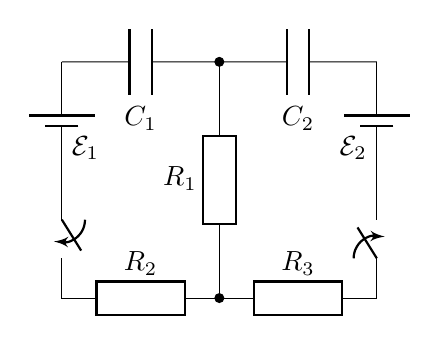
\begin{tikzpicture}[european]
	\draw (0,3) to [battery1] (0, 1.5) to [switch] (0,0) to [R=$R_2$, -*] (2,0) to [R = $R_3$] (4,0) to [switch] (4,1.5);
	\draw (4,3) to [battery1] (4, 1.5);
	\draw (4,3) to [capacitor=$C_2$, -*] (2,3) to [capacitor=$C_1$] (0,3); 	
	\node at (0.3,1.9) {$\mathcal{E}_1$};
	\node at (3.7,1.9) {$\mathcal{E}_2$};
	\draw (2,0) to [R=$R_1$] (2,3);
\end{tikzpicture}
\end{document}